
\documentclass{exam}

\usepackage{units} 
\usepackage{graphicx}
\usepackage[fleqn]{amsmath}
\usepackage{cancel}
\usepackage{float}
\usepackage{mdwlist}
\usepackage{booktabs}
\usepackage{cancel}
\usepackage{polynom}
\usepackage{caption}
\usepackage{fullpage}
\usepackage{xfrac}
\usepackage{enumerate}

\newcommand{\degree}{\ensuremath{^\circ}} 
\everymath{\displaystyle}

% \begin{figure}[h]
%   \centering
%   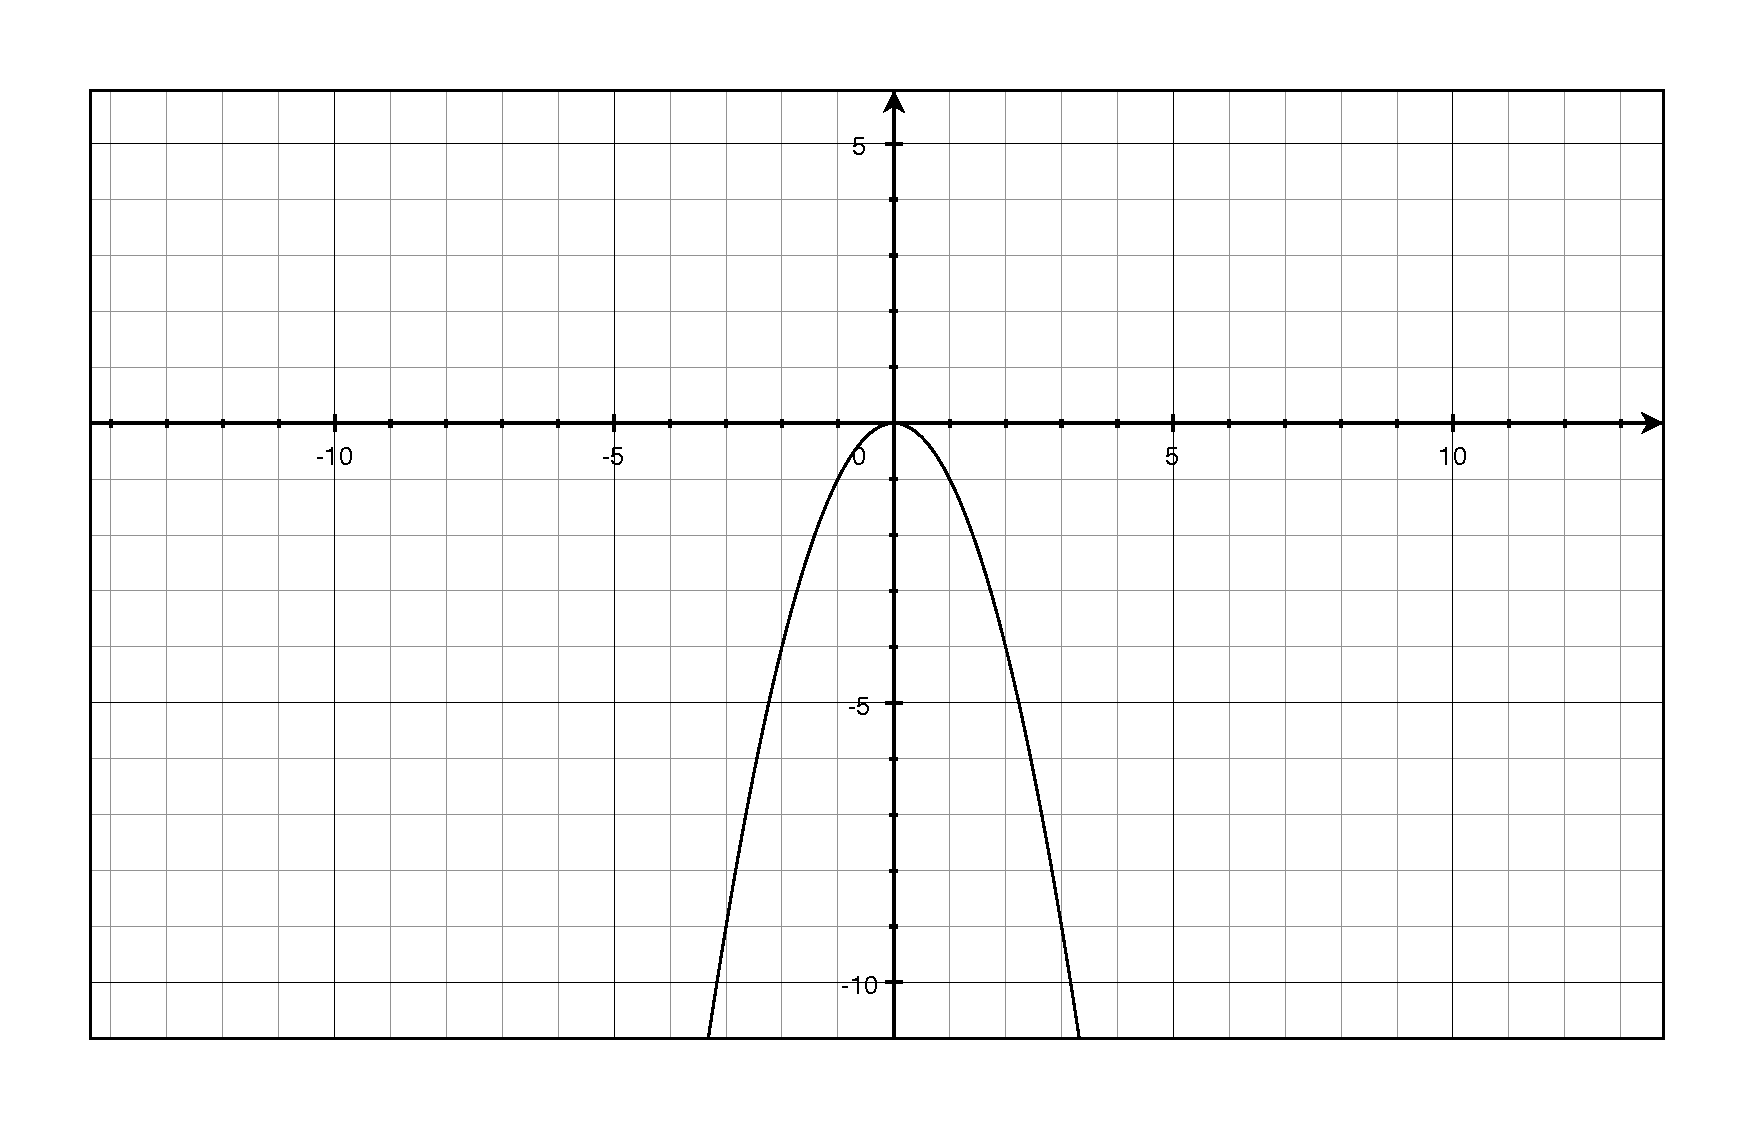
\includegraphics[scale=.3]{problem7.eps}
%   \caption*{problem 7}
% \end{figure}

% \begin{tabular}{cc}
%   \toprule
%   period & amplitude \\
%   \midrule
%   value one & value two
%   \bottomrule
% \end{tabular}

\printanswers

\ifprintanswers 
  \usepackage{2in1, lscape} 
\fi

\date{April 17, 2013}
\author{}
\title{Math 141 \\ Homework 9}

\begin{document}

  \maketitle

  \section{Homework}

  \begin{itemize*}
    \item Read Section 3.3
    \item Section 3.3: 1-10, 15-19, 30-31, 34-36, 41-44, 47, 51-52, 55, 59, 60-66, 73-74 
  \end{itemize*}

  \section{Extra Credit}
  Section 3.3, problem 100

  \begin{solution}
    \begin{enumerate}[a]
      \item Every polynomial of degree three must cross the x-axis at least once because the end behavior is to go
        towards $\pm \infty$.  So there aren't any polynomials of degree three with no real zeros.

      \item $P(x) = x^2 + 1$.  You just have to make sure that you only include even powers and include a positive
        constant term.

      \item 
        \begin{align*}
          P(x) &= x(x + \sqrt{2})(x - \sqrt{2}) \\
               &= x(x^2 - 2) \\
               &= x^3 - 2x \\
        \end{align*}
        You have to make the two irrational solutions a difference of two squares pair.

      \item
        \begin{align*}
          P(x) &= (x + \sqrt{2})(x - \sqrt{2})(x + \sqrt{3})(x - \sqrt{3}) \\
               &= (x^2 - 2)(x^2 - 3) \\
               &= x^4 - 5x^2 + 6 \\
        \end{align*}
        You have to make each of the two irrational solutions a difference of two squares pair.

      \item It must be even degree.  Any polynomial of odd degree will eventually cross the x-axis.

    \end{enumerate}
  \end{solution}

  \ifprintanswers
    \pagebreak
  \fi

  \section{Review}
  \begin{enumerate}
    \item $P(x) = x^3 - 3x^2$.  What is the average rate of change of $f$ between $x = 2$ and $x = 5$?
      \begin{solution}
        \[ 
          avg = \frac{f(5) - f(2)}{5 - 2} = \frac{50 - (-4)}{3} = 18
        \]
      \end{solution}

    \item An aquarium with an open top and a height $\unit[1.5]{ft}$ is to have a volume of $\unit[6]{ft^3}$.  Let $x$
      denote the length of the base and $y$ the width of the base.

      \begin{parts}
        \part Express $y$ as a function of $x$.

        \begin{solution}
          Since the desired volume is $\unit[6]{ft^3}$:
          \begin{align*}
            6 &= \frac{3}{2} xy \\
            y &= \frac{4}{x} \\
          \end{align*}
        \end{solution}

        \part Express the number of square feet of glass needed, $S$, as a function of $x$.
          \begin{solution}
            \begin{itemize}
              \item The area of one pair of sides is $2 \cdot \frac{3}{2} x = 3x$ 
                
              \item The area of the other pair of sides is $2 \cdot \frac{3}{2} y = 3y$ 

              \item The area of the base is $xy$

              \item The total area of glass is: $A = 3x + 3y + xy$ 
            \end{itemize}

            Plug in the answer from part (a) to express the area as a function of $x$
            \begin{align*}
              A &= 3x + 3 \left( \frac{4}{x} \right) + x \left( \frac{4}{x} \right) \\
                &= 3x + \frac{12}{x} + 4 \\
            \end{align*}

          \end{solution}
        \end{parts}

      \item
        An object is projected vertically upward from the top of a building with an initial velocity of
        $\unit[144]{ft/sec}$.  Its distance, $s(t)$ in feet above the ground after $t$ seconds is given by the equation:
        \[
          s(t) = -16t^2 + 144t + 100
        \]

        \begin{parts}
          \part Find the object's maximum distance above the ground.
            \begin{solution}
              The maximum value occurs at 
              \begin{align*}
                t &= \frac{-b}{2a} \\
                  &= \frac{-144}{2 \cdot (-16)} \\
                  &= \unit[4.5]{s} \\
              \end{align*}
              
              The height of the object at $t = \unit[4.5]{s}$ is:
              \[
                s(4.5) = \unit[424]{ft}
              \]

            \end{solution}

          \part Find the height of the building.
            \begin{solution}
              The height of the building is the height of the object at $t = \unit[0]{s}$:
              \[
                s(0) = \unit[100]{ft}
              \]
            \end{solution}
        \end{parts}

    \end{enumerate}

  \ifprintanswers
    \pagebreak

    \section{Section 3.3}

    \begin{description}

      \item[1] $\{\pm 1, \pm 3 \}$

      \item[2] $\{\pm 1, \pm 2, \pm 4, \pm 8 \}$

      \item[3] $\left\{ \pm \frac{1}{2}, \pm 1, \pm 2, \pm 4, \pm 8 \right\}$

      \item[4] 
        $\left\{ \pm \frac{1}{6}, \pm \frac{1}{3}, \pm \frac{1}{2}, \pm \frac{2}{3}, \pm 1, \pm \frac{4}{3}, 
          \pm \frac{3}{2}, \pm 2, \pm 3, \pm 4, \pm 6, \pm 12 \right\}$

      \item[5] $\left\{ \frac{1}{4}, \pm \frac{1}{2}, \pm 1, \pm \frac{7}{4}, \pm \frac{7}{2}, \pm 7 \right\}$

      \item[6] 
        If you just start with the original equation, the possibilities are:
        \[
          \left\{ \pm \frac{1}{12}, \pm \frac{1}{6}, \pm \frac{1}{4}, \pm \frac{1}{3}, \pm \frac{1}{2}, 
          \pm \frac{2}{3}, \pm 1, \pm \frac{4}{3}, \pm 2, \pm \frac{8}{3}, \pm 4, \pm 8 \right\}
        \]

        It's a little easier if you notice that you can factor 2 out of the original equation:
        \[
          12x^5 + 6x^3 - 2x - 8 = 2(6x^5 + 3x^3 - x - 4)
        \]
        which leaves the possibilities:
        \[
          \left\{ \pm \frac{1}{6}, \pm \frac{1}{3}, \pm \frac{1}{2}, 
          \pm \frac{2}{3}, \pm 1, \pm \frac{4}{3}, \pm 2, \pm 4 \right\}
        \]

      \item[7]
        \begin{tabular}{ll}
          \toprule
          Candidates & $\left\{ \pm \frac{1}{5}, \pm 1 \right\}$ \\
          \midrule
          Zeros      & $\left\{ -1, \frac{1}{5}, 1 \right\}$ \\
          \bottomrule
        \end{tabular}

        \vspace{.5 cm}

      \item[8]

        \begin{tabular}{ll}
          \toprule
          Candidates & $\left\{ \frac{1}{3}, \pm \frac{2}{3}, \pm 1, \pm 2 \right\}$ \\
          \midrule
          Zeros      & $\left\{ -1, \frac{2}{3} \right\}$ \\
          \bottomrule
        \end{tabular}

        \vspace{.5 cm}

      \item[9]
        \begin{tabular}{ll}
          \toprule
          Candidates & $\left\{ \pm \frac{1}{2}, \pm 1, \pm \frac{3}{2}, \pm 3 \right\}$ \\
          \midrule
          Zeros      & $\left\{ -\frac{1}{2}, 1, 3 \right\}$ \\
          \bottomrule
        \end{tabular}

        \vspace{.5 cm}

      \item[10]
        \begin{tabular}{ll}
          \toprule
          Candidates & $\left\{ \pm \frac{1}{4}, \pm \frac{1}{2}, \pm 1 \right\}$ \\
          \midrule
          Zeros      & $\left\{ \frac{1}{4}, 1 \right\}$ \\
          \bottomrule
        \end{tabular}

        \vspace{.5 cm}

      \item[15]
        \begin{align*}
          P(x) &= x^3 - 6x^2 +12x - 8 \\
               &= (x - 2)^3 \\
        \end{align*}

        \begin{tabular}{ll}
          \toprule
          Candidates & $\left\{ \pm 1, \pm  2, \pm  4, \pm  8 \right\}$ \\
          \midrule
          Zeros      & $\left\{ 2 \right\}$ \\
          \bottomrule
        \end{tabular}

        \vspace{.5 cm}

      \item[16]
        \begin{align*}
          P(x) &= x^3 - x^2 - 8x + 12 \\
               &= (x + 2)(x^2 - 4x + 4) \\
               &= (x + 3)(x - 2)^2 \\
        \end{align*}

        \begin{tabular}{ll}
          \toprule
          Candidates & $\left\{ \pm 1, \pm 2, \pm 3, \pm 4, \pm 6, \pm 12 \right\}$ \\
          \midrule
          Zeros      & $\left\{ -3, 2 \right\}$ \\
          \bottomrule
        \end{tabular}

        \vspace{.5 cm}

      \item[17]
        \begin{align*}
          P(x) &= x^3 - 4x^2 + x + 6 \\
               &= (x + 1)(x^2 - 5x + 6) \\
               &= (x + 1)(x - 2)(x - 3) \\
        \end{align*}

        \begin{tabular}{ll}
          \toprule
          Candidates & $\left\{ \pm 1, \pm 2, \pm 3, \pm 4, \pm 6 \right\}$ \\
          \midrule
          Zeros      & $\left\{ -1, 2, 3 \right\}$ \\
          \bottomrule
        \end{tabular}

        \vspace{.5 cm}

      \item[18]
        \begin{align*}
          P(x) &= x^3 - 4x^2 - 7x + 10 \\
               &= (x - 1)(x^2 - 3x - 10) \\
               &= (x - 1)(x + 2)(x - 5) \\
        \end{align*}

        \begin{tabular}{ll}
          \toprule
          Candidates & $\left\{ \pm 1, \pm 2, \pm 5, \pm 10 \right\}$ \\
          \midrule
          Zeros      & $\left\{ -2, 1, 5 \right\}$ \\
          \bottomrule
        \end{tabular}

        \vspace{.5 cm}

      \item[19]
        \begin{align*}
          P(x) &= x^3 + 3x^2 + 6x + 4 \\
               &= (x + 1)(x^2 + 2x + 4) \\
        \end{align*}

        \begin{tabular}{ll}
          \toprule
          Candidates & $\left\{ \pm 1, \pm 2, \pm 4 \right\}$ \\
          \midrule
          Zeros      & $\left\{ -1 \right\}$ \\
          \bottomrule
        \end{tabular}

        \vspace{.5 cm}

      \item[30]
        \begin{align*}
          P(x) &= 2x^3 - 3x^2 - 2x + 3 \\
               &= (x + 1)(2x^2 - 5x + 3) \\
               &= (x + 1)(2x - 3)(x - 1) \\
        \end{align*}

        \begin{tabular}{ll}
          \toprule
          Candidates & $\left\{ \pm \frac{1}{2}, \pm 1, \pm \frac{3}{2}, \pm 3 \right\}$ \\
          \midrule
          Zeros      & $\left\{ -1, \frac{3}{2}, 1 \right\}$ \\
          \bottomrule
        \end{tabular}

        \vspace{.5 cm}

      \item[31]
        \begin{align*}
          P(x) &= 4x^3 - 7x + 3 \\
               &= (x - 1)(4x^2 + 4x - 3) \\
               &= (x - 1)(2x + 3)(2x - 1) \\
        \end{align*}

        \begin{tabular}{ll}
          \toprule
          Candidates & $\left\{ \pm \frac{1}{4}, \pm \frac{1}{2}, \pm \frac{3}{4}, \pm 1, \pm \frac{3}{2}, \pm 3 \right\}$ \\
          \midrule
          Zeros      & $\left\{ -\frac{3}{2}, \frac{1}{2}, 1 \right\}$ \\
          \bottomrule
        \end{tabular}

        \vspace{.5 cm}

  %    \item[32]
  %      \begin{tabular}{ll}
  %        \toprule
  %        Candidates & $\left\{ \pm \frac{1}{8}, \pm \frac{1}{4}, \pm \frac{3}{8}, \pm \frac{1}{2}, \pm \frac{3}{4}, 
  %          \pm 1, \pm \frac{3}{2}, \pm 3 \right\}$ \\
  %        \midrule
  %        Zeros      & $\left\{ -1, -\frac{3}{4}, \frac{1}{2} \right\}$ \\
  %        \bottomrule
  %      \end{tabular}
  %
  %      \vspace{.5 cm}
   
  %    \item[33]
  %      \begin{tabular}{ll}
  %        \toprule
  %        Candidates & $\left\{ \pm \frac{1}{4}, \pm \frac{1}{2}, \pm \frac{3}{4}, \pm 1, \pm \frac{5}{4}, 
  %          \pm \frac{3}{2}, \pm \frac{5}{2}, \pm 3, \pm \frac{15}{4}, \pm 5, \pm \frac{15}{2}, \pm 15 \right\}$ \\
  %        \midrule
  %        Zeros      & $\left\{ -\frac{5}{2}, -1, \frac{3}{2} \right\}$ \\
  %        \bottomrule
  %      \end{tabular}
  %
  %      \vspace{.5 cm}

      \item[34]
        \begin{align*}
          P(x) &= 6x^3 + 11x^2 - 3x - 2 \\
               &= (x + 2)(6x^2 - x - 1) \\
               &= (x + 2)(3x + 1)(2x - 1) \\
        \end{align*}

        \begin{tabular}{ll}
          \toprule
          Candidates & $\left\{ \pm \frac{1}{6}, \pm \frac{1}{3}, \pm \frac{1}{2}, \pm \frac{2}{3}, \pm 1, \pm 2 \right\}$ \\
          \midrule
          Zeros      & $\left\{  -2, -\frac{1}{3}, \frac{1}{2} \right\}$ \\
          \bottomrule
        \end{tabular}

        \vspace{.5 cm}

    \pagebreak

      \item[35]
        \begin{align*}
          P(x) &= 2x^4 - 7x^3 + 3x^2 + 8x - 4 \\
               &= (x + 1)(2x^3 - 9x^2 +12x - 4) \\
               &= (x + 1)(x - 2)(2x^2 - 5x + 2) \\
               &= (x + 1)(x - 2)(2x - 1)(x - 2) \\
               &= (x + 1)(2x - 1)(x - 2)^2 \\
        \end{align*}

        \begin{tabular}{ll}
          \toprule
          Candidates & $\left\{ \pm \frac{1}{2}, \pm 1, \pm 2, \pm 4 \right\}$ \\
          \midrule
          Zeros      & $\left\{ -1, \frac{1}{2}, 2 \right\}$ \\
          \bottomrule
        \end{tabular}

        \vspace{.5 cm}

      \item[36]
        \begin{align*}
          P(x) &= 6x^4 - 7x^3 - 12x^2 + 3x + 2 \\
               &= (x + 1)(6x^3 - 13x^2 + x + 2) \\
               &= (x + 1)(x - 2)(6x^2 - x - 1) \\
               &= (x + 1)(x - 2)(3x + 1)(2x - 1) \\
        \end{align*}

        \begin{tabular}{ll}
          \toprule
          Candidates & $\left\{ \pm \frac{1}{2}, \pm 1, \pm 2, \pm 4 \right\}$ \\
          \midrule
          Zeros      & $\left\{ -1, - \frac{1}{3}, \frac{1}{2}, 2 \right\}$ \\
          \bottomrule
        \end{tabular}

        \vspace{.5 cm}

    \pagebreak

      \item[41] 
        \begin{align*}
          P(x) &= x^3 + 4x^2 + 3x - 2  \\
               &= (x + 2)(x^2 + 2x - 1) \\
        \end{align*}

        quadratic formula:
        \begin{align*}
          x &= \frac{-2 \pm \sqrt{4 + 4}}{2} \\
            &= -1 \pm \sqrt{2} \\
        \end{align*}

        \begin{tabular}{ll}
          \toprule
          Candidates & $\left\{ \pm 1, \pm 2 \right\}$ \\
          \midrule
          Zeros      & $\left\{ -1 \pm \sqrt{2}, -2 \right\}$ \\
          \bottomrule
        \end{tabular}

        \vspace{.5 cm}

      \item[42] 
        \begin{align*}
          P(x) &= x^3 - 5x^2 + 2x + 12 \\
               &= (x - 3)(x^2 - 2x - 4)
        \end{align*}
        
        quadratic formula:
        \begin{align*}
          x &= \frac{2 \pm \sqrt{4 + 16}}{2} \\
            &= 1 \pm \sqrt{5} \\
        \end{align*}

        \begin{tabular}{ll}
          \toprule
          Candidates & $\left\{ \pm 1, \pm 2, \pm 3, \pm 4, \pm 6, \pm 12 \right\}$ \\
          \midrule
          Zeros      & $\left\{ 1 \pm \sqrt{5}, 3 \right\}$ \\
          \bottomrule
        \end{tabular}

        \vspace{.5 cm}

    \pagebreak

      \item[43] 
        \begin{align*}
          P(x) &= x^4 - 6x^3 + 4x^2 + 15x + 4 \\
               &= (x + 1)(x^3 - 7x^2 + 11x + 4) \\
               &= (x + 1)(x + 3)(x^2 - 3x - 1) \\
        \end{align*}
        
        quadratic formula:
        \begin{align*}
          x &= \frac{3 \pm \sqrt{9 + 4}}{2} \\
            &= \frac{3 \pm \sqrt{13}}{2} \\
        \end{align*}

        \begin{tabular}{ll}
          \toprule
          Candidates & $\left\{ \pm 1, \pm 2, \pm 4 \right\}$ \\
          \midrule
          Zeros      & $\left\{ \frac{3 \pm \sqrt{13}}{2}, -1, 4 \right\}$ \\
          \bottomrule
        \end{tabular}

        \vspace{.5 cm}

      \item[44] 
        \begin{align*}
          P(x) &= x^4 + 2x^3 - 2x^2 - 3x + 2 \\
               &= (x - 1)(x^3 + 3x^2 + x - 2) \\
               &= (x + 1)(x + 2)(x^2 + x - 1) \\
        \end{align*}
        
        quadratic formula:
        \begin{align*}
          x &= \frac{-1 \pm \sqrt{1 + 4}}{2} \\
            &= \frac{-1 \pm \sqrt{5}}{2} \\
        \end{align*}

        \begin{tabular}{ll}
          \toprule
          Candidates & $\left\{ \pm 1, \pm 2 \right\}$ \\
          \midrule
          Zeros      & $\left\{ \frac{-1 \pm \sqrt{5}}{2}, -2, 1 \right\}$ \\
          \bottomrule
        \end{tabular}

        \vspace{.5 cm}

      \item[47] 
        \begin{align*}
          P(x) &= 4x^3 - 6x^2 + 1 \\
               &= \left( x - \frac{1}{2} \right)(4x^2 - 4x - 2) \\
        \end{align*}
        
        quadratic formula:
        \begin{align*}
          x &= \frac{4 \pm \sqrt{16 + 32}}{2} \\
            &= \frac{1 \pm \sqrt{3}}{2} \\
        \end{align*}

        \begin{tabular}{ll}
          \toprule
          Candidates & $\left\{ \frac{1}{4}, \pm \frac{1}{2}, \pm 1 \right\}$ \\
          \midrule
          Zeros      & $\left\{ \frac{1 \pm \sqrt{3}}{2}, \frac{1}{2} \right\}$ \\
          \bottomrule
        \end{tabular}

        \vspace{.5 cm}

    \pagebreak

      \item[51] 
        \begin{align*}
          P(x) &= x^3 - 3x^2 - 4x + 12 \\
               &= (x - 3)(x^2 - 4) \\
               &= (x - 3)(x + 2)(x - 2) \\
        \end{align*}
        
        \begin{tabular}{ll}
          \toprule
          Candidates & $\left\{ \pm 1,\pm 2,\pm 3,\pm 4,\pm 6,\pm 12 \right\}$ \\
          \midrule
          Zeros      & $\left\{ -2, 2, 3 \right\}$ \\
          \bottomrule
        \end{tabular}

        \begin{figure}[H]
          \centering
          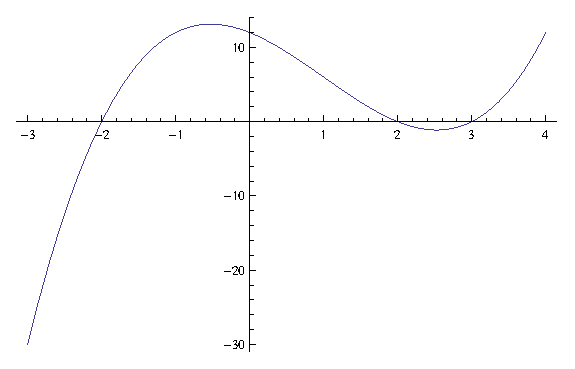
\includegraphics[scale=.9]{problem51.eps}
          \caption*{Problem 51}
        \end{figure}

    \pagebreak

      \item[52] 
        \begin{align*}
          P(x) &= -x^3 - 2x^2 + 5x + 6 \\
               &= - (x + 1)(x^2 + x - 6) \\
               &= - (x + 1)(x + 3)(x - 2) \\
        \end{align*}

        \begin{tabular}{ll}
          \toprule
          Candidates & $\left\{ \pm 1, \pm 2, \pm 9, \pm 6 \right\}$ \\
          \midrule
          Zeros      & $\left\{ -3, -1, 2 \right\}$ \\
          \bottomrule
        \end{tabular}

        \begin{figure}[H]
          \centering
          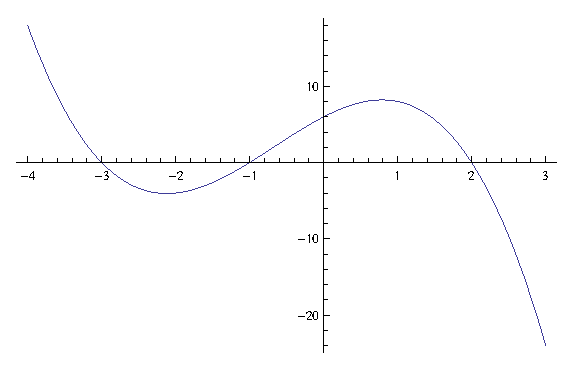
\includegraphics[scale=.9]{problem52.eps}
          \caption*{Problem 52}
        \end{figure}

    \pagebreak

      \item[55] 
        \begin{align*}
          P(x) &= x^4 - 5x^3 + 6x^2 + 4x - 8 \\
               &= (x + 1)(x^3 - 6x^2 + 12x - 8) \\
               &= (x + 1)(x - 2)^3 \\
        \end{align*}

        \begin{tabular}{ll}
          \toprule
          Candidates & $\left\{ \pm 1, \pm 2, \pm 4, \pm 8 \right\}$ \\
          \midrule
          Zeros      & $\left\{ -1, 2 \right\}$ \\
          \bottomrule
        \end{tabular}

        \begin{figure}[H]
          \centering
          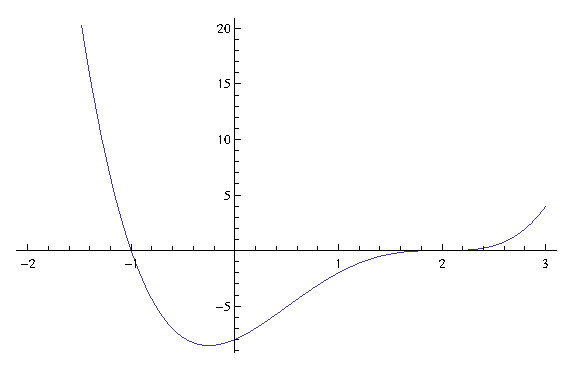
\includegraphics[scale=.9]{problem55.eps}
          \caption*{Problem 55}
        \end{figure}

      \item[59]
        $P(x) = x^3 - x^2 - x - 3$
        \begin{itemize*}
          \item 1 positive real zero
          \item 2 or 0 negative real zeros
          \item 3 or 1 real zeros
        \end{itemize*}
        
      \item[60]
        $P(x) = 2x^6 + 5x^4 - x^3 - 5x - 1$
        \begin{itemize*}
          \item 3 or 1 positive real zeros
          \item no negative real zeros
          \item 3 or 1 real zeros
        \end{itemize*}

      \pagebreak

      \item[61]
        $P(x) = 2x^6 + 5x^4 - x^3 - 5x - 1$
        \begin{itemize*}
          \item 1 positive real zero
          \item 1 negative real zero
          \item 2 real zeros
        \end{itemize*}
        
      \item[62]
        $P(x) = x^4 + x^3 + x^2 + x + 12$

        \begin{itemize*}
          \item no positive real zeros
          \item 4, 2, or 0 negative real zeros
          \item 4, 2, or 0 real zeros
        \end{itemize*}
          
      \item[63]
        For this one, $x = 0$ is one of the real zeros:
        \begin{align*}
          P(x) &= x^5 + 4x^3 - x^2 + 6x \\
               &= x(x^4 + 4x^2 - x + 6) \\
        \end{align*}

        Use the rule of signs to determine how many more real zeros there are, besids $x = 0$:
        \begin{itemize*}
          \item 2 or 0 positive real zeros
          \item no negative real zeros
          \item Including $x = 0$, there are there are 3 or 1 real zeros
        \end{itemize*}
          
      \item[64]
        $P(x) = x^8 - x^5 + x^4 - x^3 + x^2 - x + 1$

        \begin{itemize*}
          \item 6, 4, 2, or 0 positive real zeros
          \item no negative real zeros
          \item 6, 4, 2, or 0 real zeros
        \end{itemize*}

    \pagebreak

      \item[65]
        $\polyhornerscheme[x = -3]{2x^3 + 5x^2 + x - 2}$

        $\polyhornerscheme[x = 1]{2x^3 + 5x^2 + x - 2}$

      \item[66]
        $\polyhornerscheme[x = -3]{x^4 - 2x^2 - 9x^2 + 2x + 8}$

        $\polyhornerscheme[x = 5]{x^4 - 2x^2 - 9x^2 + 2x + 8}$

      \item[73]
        The candidate roots are: $\left\{\frac{1}{2}, \pm 1, \pm 2\right\}$
        
        \begin{align*}
          P(x) &= 2x^4 + 3x^3 - 4x^2 - 3x + 2 \\
               &= (x - 1)(2x^3 + 5x^2 + x - 2) \\
               &= (x - 1)(x + 1)(2x^2 + 3x - 2) \\
               &= (x - 1)(x + 1)(2x^2 + 3x - 2) \\
               &= (x - 1)(x + 1)(2x - 1)(x + 2) \\
               \\
          x    &= \left\{ -2, -1, 1, \frac{1}{2} \right\} \\
        \end{align*}

    \pagebreak

      \item[74]
        The candidate roots are: $\left\{\frac{1}{2}, \pm 1, \pm 2\right\}$
        
        \begin{align*}
          P(x) &= 2x^4 + 15x^3 + 31x^2 + 20x + 4 \\
               &= (x + 2)(2x^3 + 11x^2 + 9x + 2) \\
               &= (x + 2)\left( x + \frac{1}{2} \right)(2x^2 + 10x + 4) \\
        \end{align*}

        The remaining quadratic equation doesn't factor, so we have to use the quadratic formula to get the last two
        roots:
        \begin{align*}
          x &= \frac{-10 \pm \sqrt{100 - 32}}{4} \\
            &= \frac{-5 \pm \sqrt{17}}{2} \\
        \end{align*}

        The roots are: $\left\{ -2, -\frac{1}{2}, \frac{-5 \pm \sqrt{17}}{2} \right\}$

    \end{description}

  \else
    \vspace{2 cm}
    \begin{quote}
      \begin{em}
        The ideally non-violent state will be an ordered anarchy. That state is the best governed which is governed the
        least.
      \end{em}
    \end{quote}

    \hspace{1 cm} --Mahatma Gandhi

  \fi

\end{document}

